\documentclass{article}
\usepackage[T1]{fontenc}
\usepackage[francais]{babel}

% Set page size and margins
% Replace `letterpaper' with`a4paper' for UK/EU standard size
\usepackage[a4paper,top=2cm,bottom=2cm,left=3cm,right=3cm,marginparwidth=1.75cm]{geometry}

% Useful packages
\usepackage{amsmath}
\usepackage{graphicx}

\usepackage{fancyhdr}
\pagestyle{fancy}

\usepackage{hyperref}
\hypersetup{
    colorlinks,
    citecolor=black,
    filecolor=black,
    linkcolor=black,
    urlcolor=black
}

\usepackage{glossaries}


\makenoidxglossaries


\loadglsentries{lexique}


%\renewcommand{\contentsname}{Table des matières}

\usepackage{xcolor}

\usepackage{eso-pic}
\usepackage{tikz}
\usepackage{float}

\usepackage{soul}
\usepackage{listings}
\newcommand{\hilight}{\makebox[0pt][s]{\color{green!50}\rule[-3.5pt]{1.0\linewidth}{11pt}}}


\usepackage{tikz}



\lstset{
    language=C,
    basicstyle=\ttfamily\small,
    keywordstyle=\color{blue}\bfseries,
    commentstyle=\color{green!40!black},
    stringstyle=\color{orange},
    showstringspaces=false,
    breaklines=true,
    numbers=left,
    numberstyle=\tiny,
    numbersep=5pt,
    frame=tb,
    framexleftmargin=16pt,
    framexrightmargin=0pt,
    xleftmargin=16pt,
    backgroundcolor=\color{gray!10},
    tabsize=2
    }


\renewcommand{\epsilon}{\varepsilon} 
\renewcommand{\phi}{\varphi} 
\title{Rapport de stage Ingénieur \\-\\Implémentation d'un ordonnanceur temps réel sur
plateforme multi-cœur hétérogène\\-}
\author{BELPOIS Vincent}

\begin{document}
    \date{2023}
    \maketitle
    \thispagestyle{empty}
    
    \vspace{10mm}
    
    \begin{center}
        
\includegraphics[width = 6cm]{Images/logo_ensma.png}
    \end{center}
    \vspace{2cm}
    \begin{center}
        
\includegraphics[width = 6cm]{Images/logo_LIAS.png}
    \end{center}
    \newpage
    \tableofcontents

    
    \AddToShipoutPictureBG{%
     \put(5,5){
\includegraphics[scale = 0.02]{Images/logo_ensma.png}}
     \put(90,5){
\includegraphics[scale = 0.08]{Images/logo_LIAS.png}}

    }
    \newpage
    
    
\section*{Présentation du stage}
\addcontentsline{toc}{section}{Présentation du stage}
\subsection{Le L.I.A.S.}
\subsection{Le sujet du stage}
\newpage

\section{Le noyau Linux}

\newpage
\section{LITMUS\textsuperscript{RT}}
\subsection{Présentation de LITMUST\textsuperscript{RT}}

\subsection{Présentation de \textit{feather-trace}}

\subsection{Implémentation d'un ordonanceur EDF partitioné}

Le but du stage étant l'implémentation d'algorithmes d'ordonnancement sur plateforme hétérogène avec migration de tâches et de jobs entre les différent \gls{processeur}, il faudra être capable de réalise des \glspl{preemption} de jobs (une exécution de tâche), les migrer, assurer le traitement d'égalités et bien d'autre problèmes.


\subsubsection{Algorithme considéré}

On cherche alors, pour commencer, à implémenter un algorithme d'ordonnancement simple afin de se familiariser avec les méthodes et fonctions fourni par \litmus. J'ai donc choisi un algorithme partitionné pour la simplicité d'ordonnancement par \gls{processeur} que cela offre. Un algorithme EDF (\textit{Earliest Deadline First}) est alors choisi pour la simplicité du choix de la tâche a exécuter. Comme son nom l'indique, on choisi à chaque instant la tâche ayant l'échéance la plus proche. On nommera par la suite cet algorithme P-EDF (\textit{Partitionned Earliest Deadline First}).

Cet algorithme à aussi été choisi car il existe un tutoriel présent sur le site \href{https://litmus-rt.org}{litmus-rt.org} détaillant la plupart des fonctions nécessaires. 


Pour montrer le fonctionnement de cet algorithme, si l'on se place sur un même \gls{processeur}, on peut visualiser l'exécution de deux tâche periodiques : 
\begin{figure}[H]
    \center
    \begin{tikzpicture}[xscale=0.5, yscale=0.6]

        \newcommand\duration{15}
        \newcommand\TaskNum{2}

        % Define task properties

        \newcommand{\rectangles}[5]{
            \expandafter\def\csname rect#1ROW\endcsname{#2}
            \expandafter\def\csname rect#1START\endcsname{#3}
            \expandafter\def\csname rect#1END\endcsname{#4}
            \expandafter\def\csname rect#1COLOR\endcsname{#5}
        }

        \newcommand{\wakeup}[3]{
            \expandafter\def\csname wakeup#1ROW\endcsname{#2}
            \expandafter\def\csname wakeup#1TIME\endcsname{#3}
        }

        \newcommand{\deadlinee}[3]{
            \expandafter\def\csname deadline#1ROW\endcsname{#2}
            \expandafter\def\csname deadline#1TIME\endcsname{#3}
        }

        \newcommand{\execEnd}[3]{
            \expandafter\def\csname execEnd#1ROW\endcsname{#2}
            \expandafter\def\csname execEnd#1TIME\endcsname{#3}
        }
        
        
        
        \rectangles{0}{0}{0}{2}{"red"}
        \rectangles{1}{0}{5}{7}{"red"}
        \rectangles{2}{0}{10}{12}{"red"}
        
        \rectangles{3}{1}{2}{5}{"red"}
        \rectangles{4}{1}{7}{8}{"red"}
        
        
        
        \wakeup{0}{0}{0}
        \wakeup{1}{1}{0}
        \wakeup{4}{0}{5}

        \wakeup{5}{0}{5}
        \wakeup{2}{0}{5}
        \wakeup{3}{0}{10}

        \deadlinee{0}{0}{5}
        \deadlinee{1}{0}{5}
        \deadlinee{2}{0}{5}
        \deadlinee{3}{0}{10}
        \deadlinee{4}{0}{15}
        \deadlinee{5}{1}{15}

        \execEnd{0}{0}{2}
        \execEnd{1}{0}{7}
        \execEnd{2}{0}{12}
        \execEnd{3}{1}{8}        
        
        
        \foreach \rect in {0,...,4}{
            \pgfmathsetmacro{\row}{\csname rect\rect ROW\endcsname}
            \pgfmathsetmacro{\start}{\csname rect\rect START\endcsname}
            \pgfmathsetmacro{\end}{\csname rect\rect END\endcsname}
            \pgfmathsetmacro{\color}{\csname rect\rect COLOR\endcsname}

            \draw[fill=\color!30] (\start,1.5*\TaskNum - 0.5 - 1.5*\row) rectangle (\end,1.5*\TaskNum -1.5 - 1.5*\row) node[midway] {};
        }

        \foreach \wake in {0,...,5}{
            \pgfmathsetmacro{\row}{\csname wakeup\wake ROW\endcsname}
            \pgfmathsetmacro{\time}{\csname wakeup\wake TIME\endcsname}
            
            \draw[stealth-, thick] (\time,1.5*\TaskNum - 0.5 - 1.5*\row + 0.15) -- (\time,1.5*\TaskNum -1.5 - 1.5*\row) node[midway, left] {};
        }

        \foreach \dead in {0,...,5}{
            \pgfmathsetmacro{\row}{\csname deadline\dead ROW\endcsname}
            \pgfmathsetmacro{\time}{\csname deadline\dead TIME\endcsname}
            
            \draw[-stealth, thick] (\time,1.5*\TaskNum - 0.5 - 1.5*\row) -- (\time,1.5*\TaskNum -1.5 - 1.5*\row-0.15) node[midway, left] {};
        }

        \foreach \end in {0,...,3}{
            \pgfmathsetmacro{\row}{\csname execEnd\end ROW\endcsname}
            \pgfmathsetmacro{\time}{\csname execEnd\end TIME\endcsname}
            
            \draw[|-, thick] (\time,1.5*\TaskNum - 0.5 - 1.5*\row + 0.15) -- (\time,1.5*\TaskNum -1.5 - 1.5*\row) node[midway, left] {};
        }
        
        
        % Axes
        \draw[->] (0,0) -- (\duration + 1,0) node[right] {Temps};
        \draw[->] (0,0) -- (0,\TaskNum*1.5) node[above] {Taches};
        
        % Time ticks
        \foreach \x in {0,1,...,\duration}
            \draw (\x,0.1) -- (\x,-0.1) node[below] {\x};
        
            \node[left] at (-0.5,2) {$\tau_1(WCET=2,T=5)$};
            \node[left] at (-0.5,0.5) {$\tau_2(WCET=4,T=15)$};

    \end{tikzpicture}   
        
    \caption{Exemple de EDF à 2 tâches}
\end{figure}

On a ici une première tâche $\tau_1$ avec un pire temps d'exécution (\textit{Worst Case Execution Time}) de 2 et une période de 5, et une seconde tâche $\tau_2$ avec un pire temps d'exécution de 4 et une période de 15. On a alors préemption de la $\tau_2$ à $t=5$ afin d'exécuter $\tau_1$. Cela est dù au réveil de la tâche $\tau_1$ (représenté par la fleche montante), tâche qui est plus prioritaire que la tâche $\tau_2$ car l'échéance de la tâche $\tau_1$ est plus proche. 


\subsubsection{Implémentation}

La construction d'un plugin d'ordonnancement nécessite la déclaration d'un module au sens de Linux. Pour Linux un module est un élément de code qui peut être chargé dynamiquement lors de l'exécution du système d'exploitation. Un module permet alors d'étendre les fonctionnalités du noyau, il a donc ont accès aux fonctions du noyau, à ses ressources et peut aussi réaliser des appels systèmes.

Pour que notre nouvel ordonnanceur soit reconnu par le noyau Linux modifié (\litmus), il faut déclarer une fonction d'initialisation :
\begin{lstlisting}[style=cstyle]
#include <linux/module.h> // used for calling module_init()

static int __init init_p_edf(void)
{
    return 0; // indicates a successful initialisation
}

module_init(init_p_edf); // specify the entry point of the module 
\end{lstlisting} 

On peut alors enregistrer ce fichier sous le nom \lstinline{sched_p_edf.c} pour suivre la nomenclature des autres ordonnanceurs fournis avec avec \litmus. Ce fichier est enregistré dans le dossier \lstinline{llinux/litmus}. On peut alors modifier le fichier \lstinline{Makefile} de ce dossier afin de l'ajouter au fichier à compiler :

\begin{lstlisting}[style=makefilestyle]  
    obj-y = sched_p_edf.o
\end{lstlisting}    

On place notre fichier à compiler sous le mot-clé \texttt{obj-y} pour signifier que l'on veut ce module compilé et inclus lors de la compilation du noyau Linux.

Une fois le makefile modifié, la compilation de notre module sera exécutée lors de la compilation du noyau Linux à l'aide de make. La compilation du noyau est discutée dans la partie \ref{sec:compilation-linux-source}.

Il faut aussi déclarer un ensemble de fonctions propres à l'ordonnancement, comme pour l'admission de tâches, le réveil d'une tâche, la fin d'une tâche, le démarrage de l'ordonnanceur, etc. Voici l'ensemble des fonctions que j'ai déclaré pour mon ordonnanceur :
\newpage
\begin{lstlisting}[style=cstyle, caption={Déclaration des fonctions de l'ordonnanceur}, label={lst:decl-func-sched}]
static struct sched_plugin p_edf_plugin = {
    .plugin_name            = "P-EDF",
    .schedule               = p_edf_schedule,
    .task_wake_up           = p_edf_task_resume,
    .admit_task             = p_edf_admit_task,
    .task_new               = p_edf_task_new,
    .task_exit              = p_edf_task_exit,
    .get_domain_proc_info   = p_edf_get_domain_proc_info,
    .activate_plugin        = p_edf_activate_plugin,
    .deactivate_plugin      = p_edf_deactivate_plugin,
    .complete_job           = complete_job,
};
\end{lstlisting}

\litmus met à notre disposition un système d'abstraction pour ces fonctions afin que chaque ordonnanceur soit compatible avec les fonctions de \litmus.


\subsubsection{Résultats et essais}

Un algorithme partitionné nécessite le démarrage des tâches sur un processeur en particulier. Par exemple, j'ai ici démarré deux tâches \texttt{rtspin} avec \textit{liblitmus}. Les tâches \texttt{rtspin} sont des tâches dont la durée d'exécution est fixé et représente la condition de fin d'exécution de celle-ci.


Les deux tâches sont alors démarrées sur le processeur 3, comme en atteste le chiffre 3 dans les exécutions des tâches de la figure \ref{fig:edf-schedualibility-demo}L'une à un pire temps d'exécution de 2ms et une période de 5ms tandis que l'autre a un pire temps d'exécution de 4ms et une période de 7ms.

\begin{figure}[H]
    \centering
    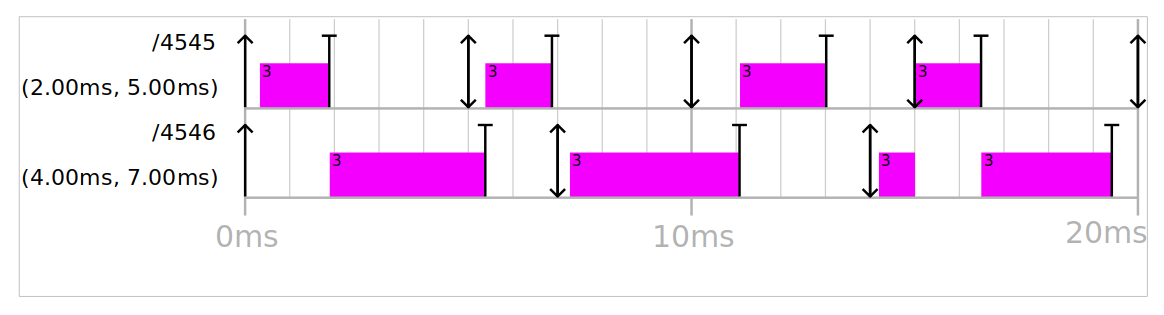
\includegraphics[width=0.95\textwidth]{Images/P-EDF-SCHEDUALIBILITY-DEMO.png}
    \caption{Ordonnancement de deux tâches avec P-EDF, toutes deux lancées sur le processeur 3}
    \label{fig:edf-schedualibility-demo}
\end{figure}

On peut voir qu'à $t=5ms$, il n'y a pas préemption de la première tâche et la seconde termine son exécution. En effet, selon EDF, la deuxième tâche à une \textit{deadline} dans 2ms, tandis que la première a une \textit{deadline} dans 5ms : la seconde est donc à cet instant plus prioritaire que la première. Cependant, à $t=15ms$, la seconde tâche est préemptée par la première car cette dernière se réveil et a une \textit{deadline} dans 5ms tandis que la seconde a une \textit{deadline} dans 6ms. On peut alors voir que la seconde tâche est préemptée à $t=15ms$ et reprend son exécution à $t=17ms$.

On remarque aussi que ce tracé n'étant pas théorique, des délais supplémentaires sont présents dù au coûts de préemption et de démarrage des tâches. On peut aussi voir que les deux tâches sont démarrées sur le même processeur, le processeur 3.
\newpage


\printnoidxglossaries

\end{document}
